%!TEX root = chap5_LVM_bayesian_main.tex
\section[Basics]{Basics on Bayesian statistics}

%###########################################################
%############################################################
\subsection{Introducing example}
\begin{frame}\frametitle{Introducing example}\label{Introduction}
\hyperlink{basics probability}{\beamerbutton{Basics in probability}}



\begin{itemize}
\item Data of Alzheimer symptoms \cite{Moran2004}
\item Presence or absence of 6 symptoms of Alzheimer's disease (AD) in 240 patients diagnosed with early onset AD conducted in the Mercer Institute in St. James's Hospital, Dublin.
\item \vert Studied symptoms\noir: Hallucination, Activity, Aggression, Agitation, Diurnal and Affective
\item \vert Final goal:\noir We want to know if we can make groups of patients suffering from the same subset of symptoms
\item\vert  HERE: \noir  \underline{we only study the presence of hallucinations}. 
\item \vert Data  \noir : 
\begin{itemize}
\item Vector of size  $n=240$ rows:   $(y_{i})_{i=1\dots n}$. 
\item $y_i=1$ denotes the presence of   hallucinations for patient $i$,  $y_i=0$ is the absence.
\end{itemize}


\end{itemize}
\end{frame}

%###########################################################
%############################################################
\begin{frame}\frametitle{$y_i$ is the realisation of a random variable $Y_i$}


\begin{block}{Assumptions} 
\noir The $Y_i$'s are independent and identically distributed
\end{block}
\begin{block}{ Statistical model: $\forall i=1\dots n$,}
 $$\left\{ 
\begin{array}{ccl}
\P(Y_i=1) &=& \theta \\
\P(Y_i=0) &=& 1-\theta  
\end{array}
\right. 
$$
$$\Updownarrow$$ $$  P(Y_i=y_i|\theta) = \theta^{y_i} (1-\theta)^{1-y_i} , y_i \in\{0,1\}
$$ 
$$\Updownarrow$$
$$
 Y_{i} \sim_{i.i.d}  \mathcal{B}ern(\theta)  
 $$
\end{block}
\begin{block}{Unknown} \centering \noir $\theta$
\end{block}

 
\end{frame}

%###########################################################
%############################################################
\begin{frame}\frametitle{First estimator of $\theta$: empirical estimator}
From the observations $y_1,\dots, y_n$: 
$$ \widehat{\theta} = \frac{\sum_{i=1}^n Y_i}{n} = \frac{n_1}{n}$$
\begin{itemize}
\item where $n_1$ is the number of individuals suffering from hallucinations 
\item \vert Here \noir  it's easy to propose one. 
\item But \vert what if \noir  one considers  a more complex model  (see later)? 
\end{itemize}
\end{frame}

%###########################################################
%############################################################
\begin{frame}[allowframebreaks]\frametitle{Second estimator: maximum likelihood}
% 
\begin{block}{Likelihood function}
  The likelihood of a (set of) parameter value(s), $\theta$, given observations $\by$  is equal to the probability of observing these data $\by$ assuming that $\theta$ was the generating parameter.   
  \end{block}
  \label{computlikbern}
  \begin{itemize}
  \item \vert Here: \noir 
  \begin{eqnarray*}
  \ell(\by; \theta)   &=&P(Y_1=y_1, \dots Y_n = y_n | \theta) \\
  &=& \prod_{i=1}^n P(Y_i=y_i | \theta)\\
  &=& \prod_{i=1}^n \theta^{Y_{i}} (1-\theta)^{1-Y_{i}} \\
  &=& \theta^{\sum_{k=1}^n Y_{i}} (1-\theta)^{\sum_{i=1}^n 1-Y_{k}}\\
  &=& \theta^{n_1} (1-\theta)^{n-n_1}\\
  \end{eqnarray*}
% %with $n_1$ the number of patients suffering from hallucinations 
 \item \vert Maximum likelihood estimator \noir  : Calculate  the ``better'' parameter $\theta$, i.e. the one maximizing the likelihood function (derivation with respect to $\theta$) 
  $$ \widehat{\theta}^{MLE}= \arg\max_{\theta}\ell(\by; \theta) $$
 \item  \vert Here \noir  maximum likelihood estimator (estimation) 
 \begin{eqnarray*} 
  \arg\max_{\theta}\ell(\by; \theta) &=& \arg\max \log \ell(\by; \theta)\\
  &=& \arg\max_{\theta} \log  \theta^{n_1} (1-\theta)^{n-n_1}\\
  &=&  \arg\max_{\theta}[ n_1  \log \theta + (n-n_1)\log (1-\theta)]
  \end{eqnarray*}
% 
\begin{eqnarray*}
 &&\frac{\partial  \log \ell(\by; \theta)}{\partial \theta}= 0  
%Leftrightarrow  \frac{\partial  [ n_1  \log \theta + (n-n_1)\log (1-\theta)]}{\partial \theta} \\
  \Leftrightarrow  \frac{n_1}{\theta} -  \frac{n- n_1}{1-\theta} = 0 \Leftrightarrow \\
 && (1-\theta) n_1 = (n-n_1)(1-\theta) \Leftrightarrow \theta = \frac{n_1}{n}
\end{eqnarray*}
% 
\vspace{1em}
% 
$$ \mbox{Estimator}:   \frac{\sum_{i=1}^n Y_i}{n}, \quad \quad \mbox{Estimation}:  \frac{\sum_{i=1}^n y_i}{n} $$
 \item  \vert Comments \noir
 \begin{itemize}
 \item Automatic estimation method 
 \item Theoretical properties well known when the number of observations $n$ is big
 \item The  maximization can be difficult
 \end{itemize}
\end{itemize}
\end{frame}


%###########################################################
%############################################################--
\begin{frame}\frametitle{Classical (frequentist) statistics: confidence interval}

 
 \begin{itemize}
 \item \vert Confidence interval\noir: finding two bounds depending on the observations such that this interval $[u(\boldsymbol{Y}), v(\boldsymbol{Y})]$ contains the true parameter $\theta$ with high probability.
 $$  \P_{\boldsymbol{Y}}\left(\theta \in [u(\boldsymbol{Y}),v(\boldsymbol{Y})]\right) = 1- \alpha$$ 
  
 
\item \vert Here \noir: 

$$\P_{\boldsymbol{Y}}\left(p \in \left[\widehat{\theta} - \frac{q_{0.05/2}}{\sqrt{n}} \sqrt{ \widehat{p}(1- \widehat{\theta})}, \widehat{\theta} + \frac{q_{0.05/2}}{\sqrt{n}} \sqrt{\widehat{\theta}(1- \widehat{\theta})} \right]\right) = 0.95 $$
\item \vert Interpretation \noir  (wikipedia) \textit{``There is a $(1-\alpha)\%$ probability that the calculated confidence interval from some future experiment encompasses the true value of the population parameter $\theta$.''}

\item It is a probability over $\boldsymbol{Y}$ : $\boldsymbol{Y}$ is  random. 

 \end{itemize}
 \end{frame}

%###########################################################
%############################################################

\subsection{Prior and posterior}

\begin{frame}\frametitle{Bayesian inference}
\begin{block}{Main idea}

\begin{enumerate}
\item \vert Model\noir: $\by$ is the realisation of $\by  \sim P(\boldsymbol{Y} | \theta)$
\item The unknown parameter $\theta$ is a random object and so we give him a \vert prior probability distribution \noir : 
$$\theta \sim \pi(\theta)$$ 
\item  Remember the \vert Bayes Formula:  \noir 
$$ \P( B | A ) = \frac{\P( A| B ) \P(B)}{\P(A)}$$  
$$ \theta \leftrightarrow B \quad \quad  \by \leftrightarrow A $$
$$ p(\theta | \by) = \frac{P(\by | \theta)\pi(\theta)}{P(\by)} =  \frac{\ell(\by | \theta)\pi(\theta)}{P(\by)} $$ 
\item $p(\theta | \by)$ is the \vert posterior probability distribution
\end{enumerate}
\end{block}
\end{frame}

%############################################################
\begin{frame}{Remarks about  the Bayesian evidence $P(\by)$}
$$ p(\theta | \by) = \frac{\ell(\by | \theta)\pi(\theta)}{P(\by)} $$ 

\begin{itemize}
\item $p(\theta | \by)$ is a probability density  so its ``sum'' over all the possible values of $\theta$ is equal to $1$ i.e. : 
$$ \int_{\theta} p(\theta | \by) d\theta  = 1$$ 
\item Leading to: 

$$ \frac{\int_{\theta}\ell(\by | \theta)\pi(\theta) d\theta}{P(\by)} =1 \Leftrightarrow   \int_{\theta}\ell(\by| \theta)\pi(\theta) d\theta = P(\by) $$ 

\item $P(\by)$ is  only a normalization constant also called the \vert marginal likelihood \noir (because it is the likelihood integrated over the prior distribution). The form on $\theta$ is given by 
$\ell(\by | \theta)\pi(\theta)$. 
\end{itemize}
\end{frame}
%###########################################################

\begin{frame}{Consequence}

 As a consequence $$p(\theta | \by)   \propto  \ell(\by | \theta)\pi(\theta) $$
 
where $\propto$ should not hide factors that depend on $\theta$
 


\vert Alternative notation \noir

$$p(\theta | \by) =  [\theta | \by] =  \frac{[\by | \theta] [\theta]}{[\by]} = \frac{\ell(\by | \theta)\pi(\theta)}{P(\by)} $$ 
 
\end{frame}
%###########################################################
\begin{frame}{First example}
 
\begin{itemize}
\item  $\theta \in [0,1]$
\item Prior distribution $$ \pi(\theta) = \ind_{[0,1]}(\theta)$$ 
\item Posterior distribution



\begin{eqnarray*}
 [\theta | \by] &=& \frac{[\by| \theta] [\theta]}{[\by]} \propto [\by | \theta] [\theta] \\
  &\propto&    \theta^{n_1} (1-\theta)^{n-n_1} \ind_{[0,1]}(\theta) \footnote{Using the likelihood computed in slide \ref{computlikbern}}\\ 
 &\propto&    \theta^{{\vert  n_1+ 1 }-1} (1-\theta)^{{\vert  n  - n_1 + 1}-1}   \ind_{[0,1]}(\theta)\\
\end{eqnarray*}

We ``recognize'' a Beta distribution (\href{https://en.wikipedia.org/wiki/Beta_distribution}{See Wikipedia})
\end{itemize} 
\end{frame}

%###########################################################

\begin{frame}[fragile]\frametitle{R Code}

\begin{verbatim}
n  <- length(Y)
n_1<- sum(Y[,1])
a <- 1
b <- 1 
curve(dbeta(x,a+n_1,b+n-n_1),0,0.4,ylab="",xlab="p",
lwd=2,col=2,ylim=c(0,20))
\end{verbatim}

\end{frame}
%###########################################################
\begin{frame}\frametitle{Posterior distributions for various $n$ }
     \begin{figure}
 \centering
 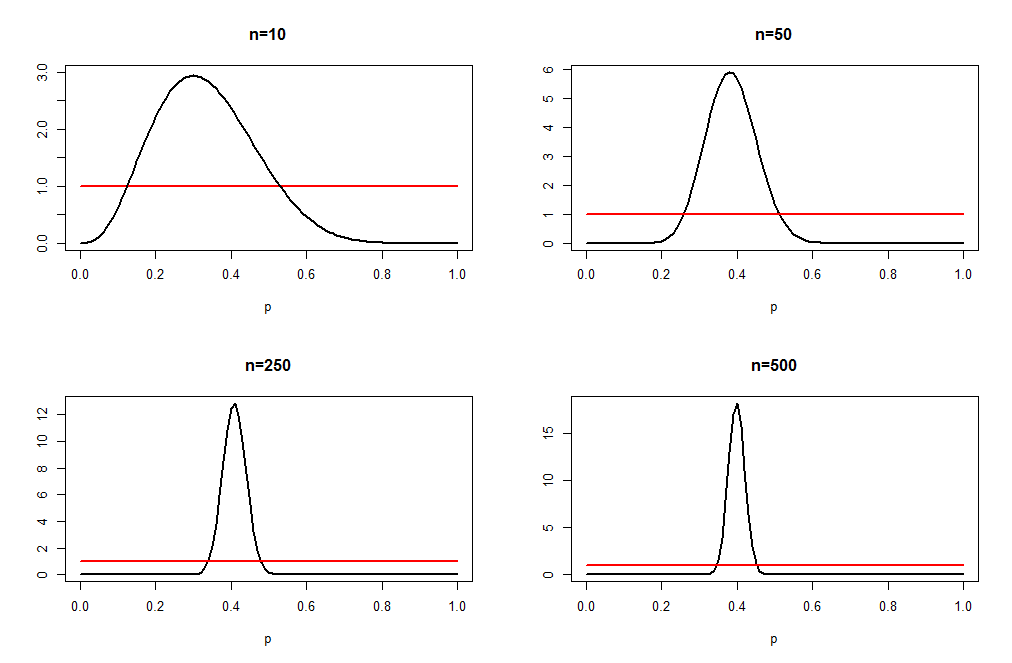
\includegraphics[width=\linewidth]{figures/post_priorunif.png}
\caption{\scriptsize Posterior densities for $\theta$,  for various sizes of the sample $n$ (prior distribution in red)}
  \end{figure}
 \end{frame}




%###########################################################
\begin{frame}\frametitle{Questions}

\begin{itemize}
 \item How to choose the prior ditribution?  
 \item  How to summarize the posterior distribution? How to do take decisions with the posterior distribution?
 \item Is it always easy to determine the posterior distribution? 
\end{itemize}

 
\end{frame}

%###########################################################

\subsection{About the prior distribution}
%###########################################################
\begin{frame}\frametitle{Choice of the prior distribution}
 \begin{columns}[t]
 \begin{column}{0.55\linewidth} 
  \begin{block}{}
\begin{itemize}
\item $\theta \in [0,1]$ :  $\theta \sim \mathcal{B}eta(a, b)$
\item $(a,b)$ are  hyperparameters
\item $ [\theta]  \propto  \theta^{a-1} (1-\theta)^{b-1} \ind_{[0,1]}(\theta)$ 
\item \vert How to chose $(a,b)$ ?  %$(a,b_k)$.  
\noir
\begin{itemize}
\item  If I don't know anything,  $a=b=1$ :  uniform distribution on $[0,1]$
 $$[\theta] \propto \ind_{[0,1]}(\theta)$$
 \item By tuning $a$ and $b$,  `` a priori'' give advantage to some values :  include  knowledge coming from previous studies or experts. 
 
% $$[\theta] \propto \prod_{k=1}^K \ind_{[0,1]}(p_k)$$
\end{itemize}
\end{itemize}
 \end{block} 
  \end{column}
  
\begin{column}{0.45\linewidth}
  \begin{block}{}
     \begin{figure}
 \centering
 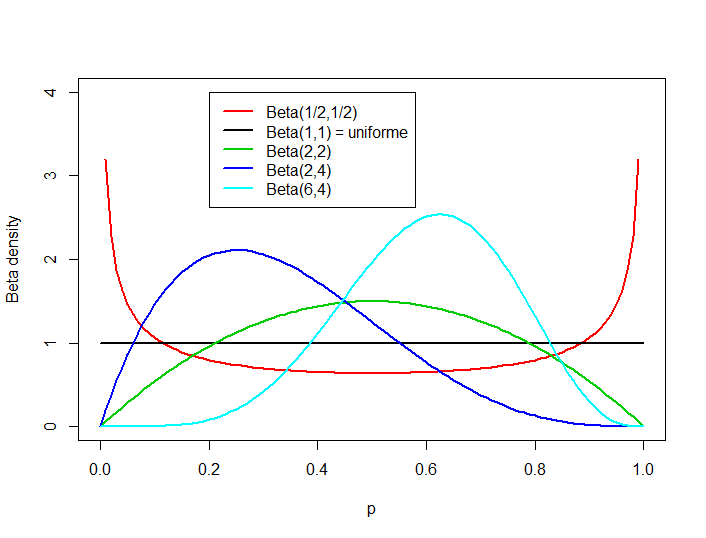
\includegraphics[width=\linewidth,height=\linewidth]{figures/plot_beta.png}
 \end{figure}
    \end{block}
  \end{column}
 \end{columns} 
\end{frame}


%###########################################################
\begin{frame}\frametitle{Posterior distribution}

\begin{eqnarray*}
 [\theta | \bY] &=& \frac{[\bY | \theta] [\theta]}{[\bY]} \propto [\bY | \theta] [\theta] \\
 &\propto&    \theta^{n_1} (1-\theta)^{n-n_1} \theta ^{a-1} (1-\theta)^{b-1}  \ind_{[0,1]}(\theta)\\ 
 &\propto&   \theta^{{\vert a+ n_1}-1} (1-\theta)^{{\vert b+n-n_1}-1}   \ind_{[0,1]}(\theta)\\
\end{eqnarray*}
We recognize 
$$\theta | \bY \sim \mathcal{B}eta(a + n_1, b+n-n_1)$$



\end{frame}

%###########################################################
\begin{frame}[fragile]\frametitle{Posterior distributions for various prior and $n$}
\centering
\begin{tabular}{cc}
   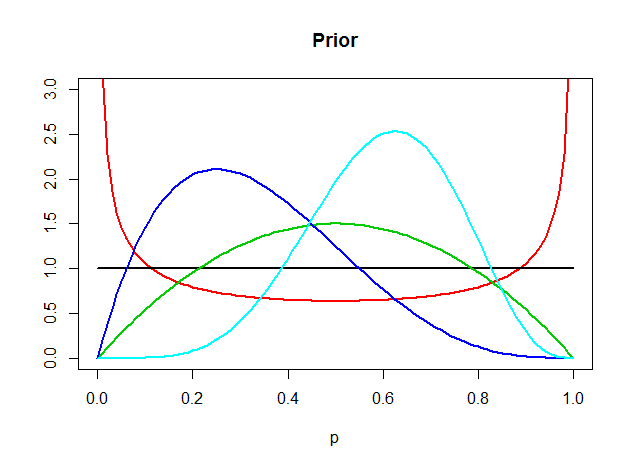
\includegraphics[width=0.4\linewidth]{figures/prior_beta.png} &
   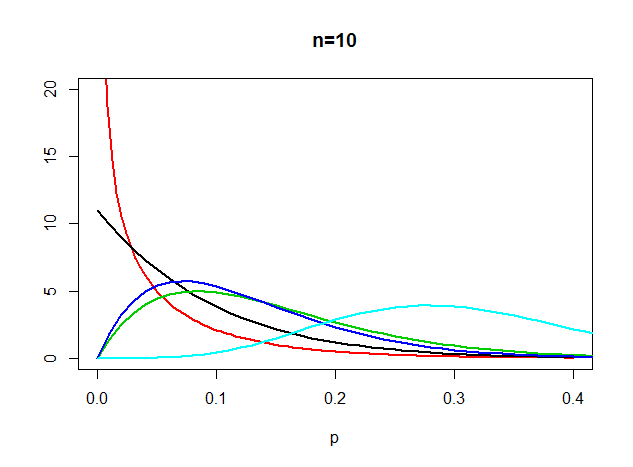
\includegraphics[width=0.4\linewidth]{figures/post_n=10.png} \\
      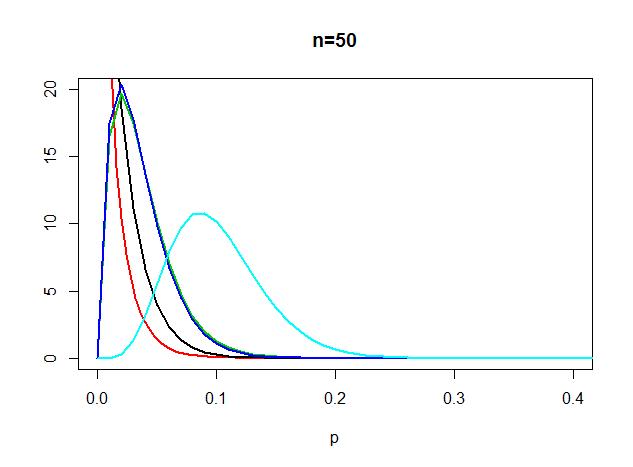
\includegraphics[width=0.4\linewidth]{figures/post_n=50.png}&
   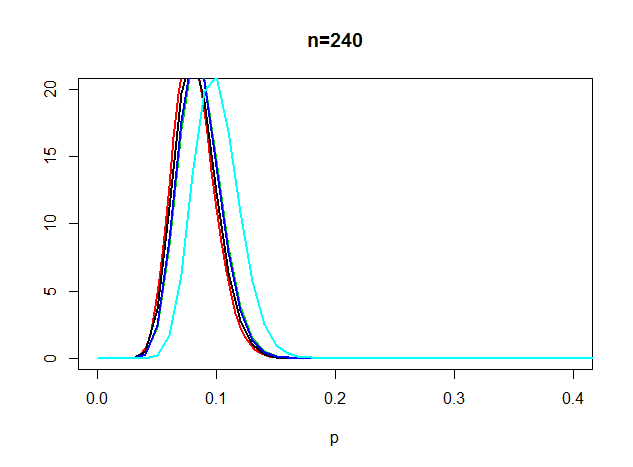
\includegraphics[width=0.4\linewidth]{figures/post_n=240.png} \\
\end{tabular}\\
\end{frame}

%###########################################################

%###########################################################
\begin{frame}\frametitle{Comments (1)}
\begin{itemize}
\item The  prior distribution on $\theta$ is updated  into a posterior distribution using the data
\item The posterior/prior distributions quantifies my incertitude on $\theta$
\item \vert Posterior\noir: compromise between the prior distribution and the data
\begin{eqnarray*}
p(\theta| \bY) &\propto& \pi(\theta) \ell(\by | \theta)\\
\log p(\theta | \by) &=& \log \pi(\theta)  +   \log \ell(\by | \theta) + C\\
\log p(\theta | \by) &=& \log \pi(\theta)  +  \sum_{i=1}^n \log \ell(y_i | \theta) + C
\end{eqnarray*}

\item The prior distribution has an influence on the posterior distribution if the number of observations $n$ is small

\item This influence vanishes if the number of observations increases 

\end{itemize}
\end{frame}
%###########################################################
\begin{frame}{Comments (2)}
 The prior distribution quantifies the prior (un)knowledge on $\theta$.
\begin{itemize} 
\item In case of complete prior incertitude : \vert non-informative prior \noir (Jeffreys: automatic construction. Improper prior) 
\item In case of external knowledge (previous experiments, experts) : \vert informative prior  
\end{itemize}
 
\end{frame}

%###########################################################
\begin{frame}\frametitle{Non informative prior}
If we do not know anything about $\theta$
  \begin{itemize}
\item Use an uniform prior as we did $\theta \sim \mathcal{U}_{[0,1]}$
\item The prior distribution can be improper  i.e $\int \pi(\theta) d \theta  = \infty$ provided the posterior distribution is a probability density
    \item Method to create an informative prior automatically:  \textbf{Jeffreys's prior}
    $$ \pi(\theta) \propto \sqrt{\det(I(\theta))}$$  where  $I(\theta)$ is the Fisher information (i.e. is big when the data contain a lot of information on the parameters )
    \begin{itemize}
    \item The prior gives more importance to values  such that  the data give a lot of informations about it:  minimizes the influence of the prior
    \end{itemize}
\end{itemize}
 
  
\end{frame}
%###########################################################

\subsection{Summary of the posterior distribution}

%###########################################################

\begin{frame}{Statistics for decisions}
 From my posterior distribution
 \begin{center}
 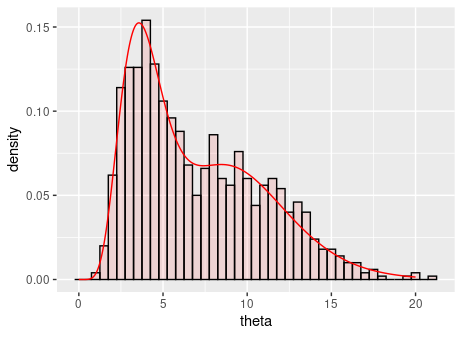
\includegraphics[width = 0.7 \textwidth]{figures/approx_post_MC.png}
 \end{center}
 
 \begin{multicols}{2}
    \begin{itemize}
      \item Parameter estimation
  \item Credible interval
  \item Hypothesis testing \footnote{\label{HOTS}Not evoked here}
  \item Model selection$^2$
    \end{itemize}
    \end{multicols}
   
 
\end{frame}


%###########################################################
\subsubsection{Estimation}
%###########################################################
 \begin{frame}\frametitle{Bayesian estimator}
 \begin{block}{Aim}
 Give an estimated value to $\theta$
 \end{block}
 
 Once we have the posterior distribution: 
 \begin{itemize}
 \item \vert Posterior expectation: \noir  $$E[\theta | \bY] = \int_{\theta} \theta [\theta | \bY]d\theta$$
 \item \vert Posterior median: \noir $$\P(\theta \leq q_{0.5} | \bY) = 0.5$$  
  \item \vert Maximum a posteriori MAP: 
    \noir $\arg\max_\theta \;  [\theta | \bY]$ 
  
 {\scriptsize  \begin{eqnarray*}
  \arg\max_\theta \;  [\theta | \bY] &=& \arg\max_{\theta} \; \log \ell(\bY | \theta)  + \log \pi(\theta) - \cancel{\vert \log P(\bY)}\\
%  &=&  \arg\max_{\theta} \; \log \ell(\bY | \theta)  + \log \pi(\theta)  \\
  &=& \arg\max_{\theta} \; \log \prod_{i=1}^n \P(Y_i | \theta)   + \log \pi(\theta)  \\
  &=& \arg\max_{\theta} \; \sum_{i=1}^n \log \P(Y_i | \theta)   + \log \pi(\theta)  
      \end{eqnarray*}}
 
  \end{itemize}
 
  \end{frame}
%###########################################################

  \begin{frame}\frametitle{Bayesian estimator in our example}
$$\theta \sim \mathcal{B}eta(a,b), \quad \quad \theta | \bY \sim \mathcal{B}eta(a + n_1, b+n-n_1)$$ 

  \begin{itemize}
 
\item\vert  Posterior expectation  \noir
$$ E[ \theta  | \bY] = \frac{a + n_1}{a + n_1+ b+n-n_1} = \frac{a + n_1}{a+b+n}$$
\item \vert MAP \noir
 $$\arg\max_\theta [\theta | \bY] =  \frac{a + n_1 - 1}{a + n_1+ b+n-n_1-2} = \frac{a + n_1-1}{a+b+n-2}$$
 \item \vert Posterior median \noir : no explicit expression 
 $$\approx \frac{a + n_1 - \frac{1}{3}}{a + n_1 +  b+n-n_1 - \frac{2}{3}} =  \frac{a + n_1 - \frac{1}{3}}{a +   b+n - \frac{2}{3}}$$
\end{itemize}
 
  \end{frame}
%###########################################################
      
   
\subsubsection{Credible interval}
  
%----------------------------------------------------------------------------- 
\begin{frame}[allowframebreaks]\frametitle{Credible interval }

  \begin{block}{Aim}
 Finding the shortest (if possible)  interval such that $$\P(\theta \in [a,b] | \bY) = 1- \alpha$$
 \end{block}
 
 Several ways to define it : 
 
\begin{block}{Highest posterior density interval  (HPD)}
It is the narrowest interval, which for a unimodal distribution will involve choosing those values of highest probability density including the mode.
 $ \mathcal{C} = \{\theta;\pi(\theta  | \bY)  \geq k\} $ where $k$ is the largest number such that $\int_{\theta; \pi(\theta  | \bY) \geq k} \pi(\theta | \bY) d\theta=1- \alpha$ 
\end{block}

\begin{figure}
\centering 
 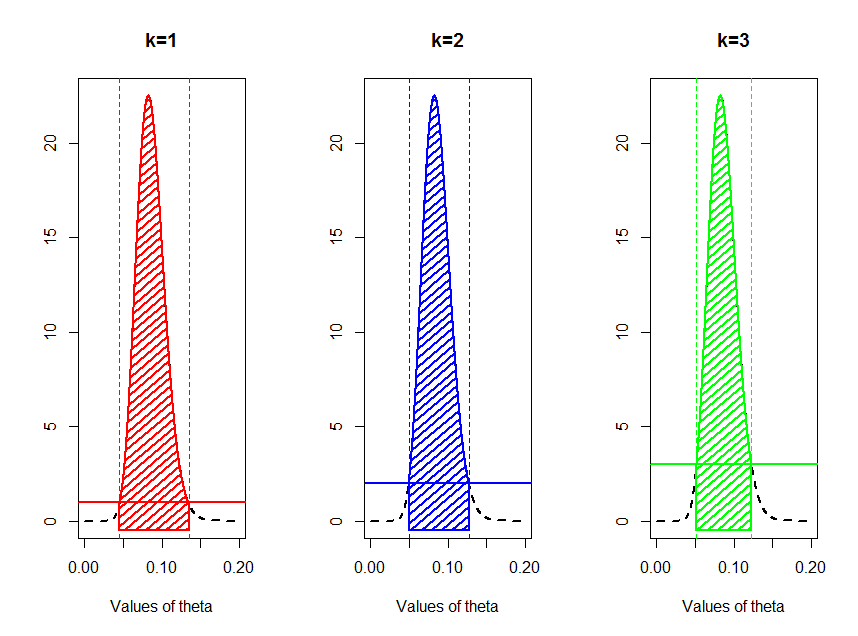
\includegraphics[width=\linewidth]{figures/HPD.png}
 \end{figure}
\end{frame}

\begin{frame}\frametitle{Highest posterior density region }

 \begin{figure}
\centering 
 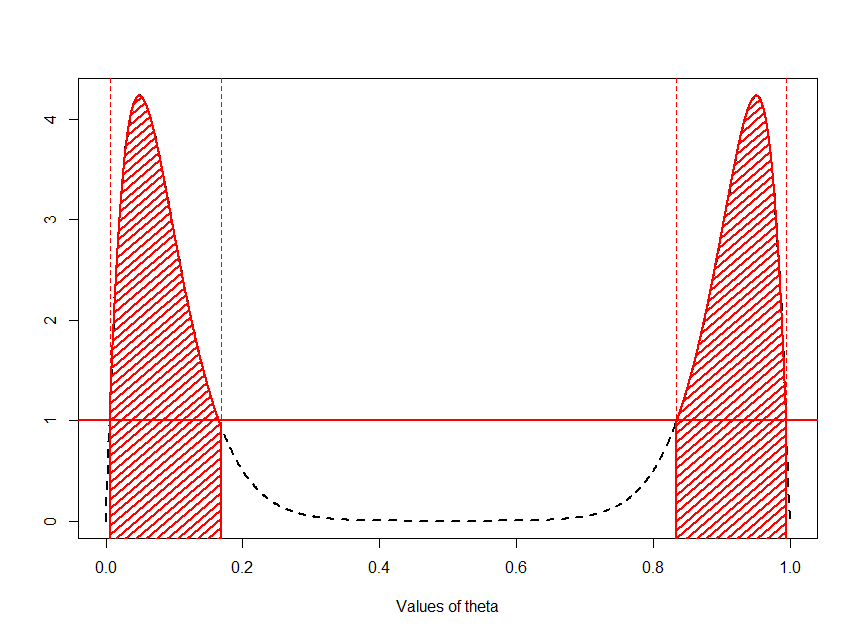
\includegraphics[width=0.6\linewidth]{figures/HPD_bimod.png}
 \end{figure}

\begin{itemize}
\item Be careful : if the posterior density is multi-modal, one can get the union of 2 intervals. 
\item Difficult to get in practice because we have to invert the density function
\end{itemize}

\end{frame}
%###########################################################
\begin{frame}

\begin{block}{Equal-tailed interval} 
Choosing the interval where the probability of being below the interval is as likely as being above it. This interval will include the median. 
\end{block}

\begin{figure}
\centering 
 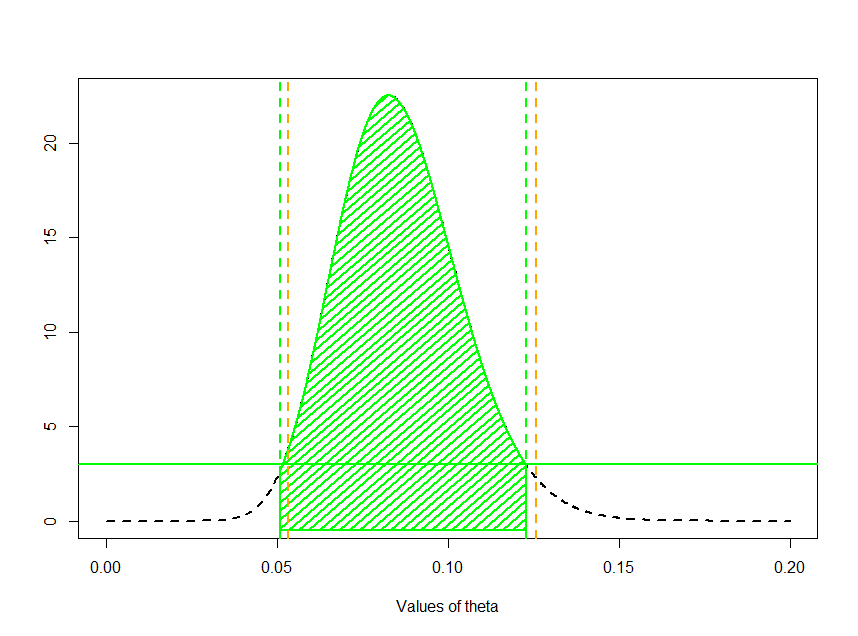
\includegraphics[width=0.8\linewidth]{figures/Equi_tailes.png}
 \end{figure}
 
  \hyperlink{BF}{\beamergotobutton{Hypothesis testing and model selection}}
 
\end{frame}
%###########################################################

%###########################################################

\begin{frame}{Take home messages}
\label{TakeHOME}
 

\begin{block}{}
\begin{itemize}
\item Bayesian statistics are only related to statistical inference (estimation, hypothesis testing...) 
\item A statistical model  is not Bayesian per se (except in neurosciences where some of them consider that the brain is ITSELF Bayesian)
\item Bayesian inference  is based on a prior distribution on the unknown quantities (parameters, models...) 
\item The prior distribution quantifies the knowledge on the unknown quantities  BEFORE the experiment. We can know nothing (non-informative prior) or  something from previous studies, from experts (informative prior). 
\item The sensibility to the prior has to be analysed to be aware of this influence
\end{itemize}
\end{block}
\end{frame}

%###########################################################

\begin{frame}{Focus on this class}
\begin{itemize}
\item Bayesian decision is a large topic. 
\item Focus of this course on the methods to obtain the posterior distribution.
\end{itemize}
 \end{frame}

%###########################################################
\subsection{Determining the posterior distribution}

\subsubsection{Conjugate case}

\begin{frame}{Conjugate prior : easy case}

In our example : beta prior \color{blue}$\rightarrow$ \color{black} beta posterior
\begin{itemize}
\item We talk about conjugate prior when the prior and the posterior distributions are in the same family 
\item \vert Examples \color{black}
\end{itemize}
$$
\begin{array}{|c|c|c|c|} 
\hline
\left[y| \theta\right]  & [\theta]  & [ \theta|y ]& \mathbb{E}[\theta|y]\\
 \hline 
 \mathcal{N}(\theta,\sigma^2)& \mathcal{N}(\mu,\tau^2)& \omega^2 = [\frac{1}{\sigma^2} + \frac{1}{\tau^2}]^{-1} & \omega^{2}(\frac{y}{\sigma^2} + \frac{\mu}{\tau^2})\\
 & &   \mathcal{N}(\omega^{2}(\frac{y}{\sigma^2} + \frac{\mu}{\tau^2}),\omega^2 )&\\
% %& & &\\
 \Gamma(n,\theta)  & \Gamma(\alpha, \beta) &   \Gamma(\alpha+y, \beta+n)& \frac{\alpha+x}{\beta+n}\\ 
% %%& & &\\
 \mathcal{B}in(n, \theta)&  \mathcal{B}(\alpha,\beta) & \mathcal{B}(\alpha + y, \beta + n - y )&  \frac{\alpha + y}{\alpha + n + \beta}\\
 \mathcal{P}(\theta) &  \Gamma(\alpha, \beta)&  \Gamma(\alpha + y, \beta + 1)&  \frac{\alpha + x}{\beta + 1}\\
 \hline
\end{array}$$
\color{dgreen}{ \footnotesize \href{https://en.wikipedia.org/wiki/Conjugate_prior}{See  Wikipedia for instance}}\color{black}

\end{frame}


%%%%%%%%%%%%%%%%%%%%%%%%%%%%%%%%%%%%%%%%%%%%%%%
\begin{frame}{To go further}

\begin{itemize}
\item For the exponential family of distributions, we have  a conjuguate prior \color{blue}$\rightarrow$ \color{black} very rare in practice
\item Note that the Gaussian regression model is congugate: 
\begin{eqnarray*}
 \bY &\sim& \mathcal{N}(X\beta,\sigma^2 \mathbb{I})\\
 \beta  | \sigma &\sim& \mathcal{N}(\beta_0,\sigma^2\Omega)
\end{eqnarray*}
Then, 


\item  For any more complex  model, (such as Latent Variable models)  the posterior distribution is not explicit
% \item People resort to 
% \begin{itemize}
%  \item Sampling methods
%  \item Approximation methods
% \end{itemize}
\end{itemize}
\end{frame}

%%%%%%%%%%%%%%%%%%%%%%%%%%%%%%%%%%%%%%%%%%%%%%%
\begin{frame}{Illustration on the mixture model}

{\footnotesize \vert In a few words\noir:  My data $y_i$ are issued from to populations, each population having its own mean. I do not know to which population each observation belongs. 
}

\begin{itemize}
 \item \vert Model \noir $Z_i \in \{1,2\}$
 \begin{eqnarray*}
 P(Z_i = 1) &=& \pi_1\\
 Y_i  | Z_i = k  &\sim&  \mathcal{N}(\mu_k,1)
 \end{eqnarray*}
\item \vert Parameters: \noir $\theta = (\pi_1,\mu_1,\mu_2)$
\item \vert Likelihood: \noir
 
\begin{eqnarray*}
[\bY | \theta] = \prod_{i=1}^n \left[\pi_1 \frac{1}{\sqrt{2\pi}}e^{-\frac{1}{2}(y_i-\mu_1)^2} + (1-\pi_1)\frac{1}{\sqrt{2\pi}}e^{-\frac{1}{2}(y_i-\mu_2)^2} \right]
\end{eqnarray*}

 
\item \vert Prior distribution: \noir
 $$\pi_1 \sim \mathcal{U}_{[0,1]}, \quad \mu_k \sim \mathcal{N}(0,\omega^2), \quad k=1,2$$
 \end{itemize}
\end{frame}

 
%----------------------------------------------------------------------------- 
\begin{frame}{Mixture distribution : posterior}

\begin{eqnarray*}
[\theta | \bY] &\propto&   [\bY | \theta] [\theta]\\
&\propto & \prod_{i=1}^n \left[\pi_1 \frac{1}{\sqrt{2\pi}}e^{-\frac{1}{2}(y_i-\mu_1)^2} + (1-\pi_1)\frac{1}{\sqrt{2\pi}}e^{-\frac{1}{2}(y_i-\mu_2)^2} \right]   \ind_{[0,1]}(\pi_1)  \\
&&  \frac{1}{\omega \sqrt{2\pi}}e^{-\frac{1}{2 \omega^2} \mu_1 ^2} \frac{1}{\omega \sqrt{2\pi}}e^{-\frac{1}{2 \omega^2} \mu_2 ^2}
\end{eqnarray*}


\begin{itemize}
\item  Non conjuguate model, posterior distribution not explicit.
\item  How to evalute, for instance the \vert posteriori mean:\noir $\int \theta [\theta | \bY] d\theta$?  
\end{itemize}
\end{frame}

 

\subsubsection{Outside the conjugate case}

%%%%%%%%%%%%%%%%%%%%%%%%%%%%%%%%%%%%%%%%%%%%%%%
\begin{frame}{How to determine a complex posterior distribution?}


\begin{itemize}
 \item Resort to algorithms to approximate the posterior distribution.
 \item 2 approaches
\begin{itemize}
 \item \vert Sampling methods\noir: supply realizations of the posterior distribution $\theta^{(1)}$, $\dots$, $\theta^{(m)}$, $\dots$, $\theta^{(M)}$.
 \item \vert Deterministic methods\noir: approximate  the density $p(\theta | \bY)$ in a given family of distribution. 
\end{itemize}
\end{itemize}
\end{frame}

%%%%%%%%%%%%%%%%%%%%%%%%%%%%%%%%%%%%%%%%%%%%%%%
\begin{frame}{Sampling methods}

\begin{block}{}
If we can simulate $\theta^{(m)} \sim_{i.i.d.} P(\theta | \by)$ for $m=1,\dots, M$, then 
$\frac{1}{M} \sum_{m=1}^M \delta_{\theta^{(m)}}(\cdot) \approx p(\cdot | \by)  $
(Glivenko-Cantelli theorem)
\end{block}

\centering
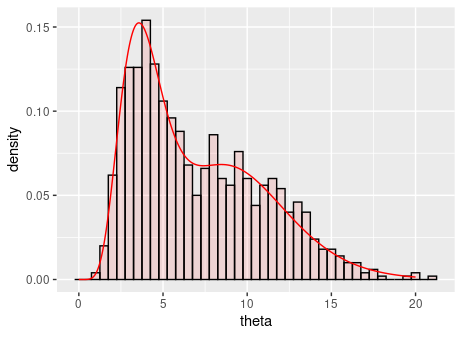
\includegraphics[width = 0.5\textwidth]{figures/approx_post_MC.png}

\begin{itemize}
\item \emph{Law of large numbers} : $\frac{1}{M} \sum_{m=1}^M  \theta^{(m)}$ approximates$^*$  $E[\theta | \by]$
\end{itemize}
\end{frame}

%%%%%%%%%%%%%%%%%%%%%%%%%%%%%%%%%%%%%%%%%%%%%%%

\begin{frame}{Monte Carlo Markov Chains methods }

Gibbs Sampler, Metropolis-Hastings algorithm...
\begin{itemize}
\item \vert\emph{Main idea}\color{black}: design a Markov Chain such that its stationary distribution is the posterior distribution
\item Generic methods
\item Supplies asymptotically realizations of the posterior distribution $\theta^{(1)}$, $\dots$, $\theta^{(m)}$, $\dots$, $\theta^{(M)}$
\item Made the success of the Bayesian inference
\end{itemize}
\end{frame}

%%%%%%%%%%%%%%%%%%%%%%%%%%%%%%%%%%%%%%%%%%%%%%%

\begin{frame}{Importance samplers}
\begin{itemize}
 \item Simulate ``particles''  $\theta^{(1)}, \dots, \theta^{(m)}, \dots, \theta^{(M)}$ with a ``simple'' distribution
  \item Give weights to the particles to correct the discrepancy between the distribution used to simulate and the posterior distribution
 \end{itemize}
\end{frame}
%%%%%%%%%%%%%%%%%%%%%%%%%%%%%%%%%%%%%%%%%%%%%%%
\begin{frame}{Deterministic approximation}

Variational Bayes for instance
 \begin{itemize}
 \item Approximate the density $p(\theta | \by)$ in a given family of distribution 
 \item Minimizes a divergence with the true posterior density.  
  \item Optimization
\end{itemize}
 

 
\end{frame}



